\documentclass[border=6mm]{standalone}
\usepackage{tikz}
\usetikzlibrary{arrows.meta,positioning,calc,fit,backgrounds}

\begin{document}
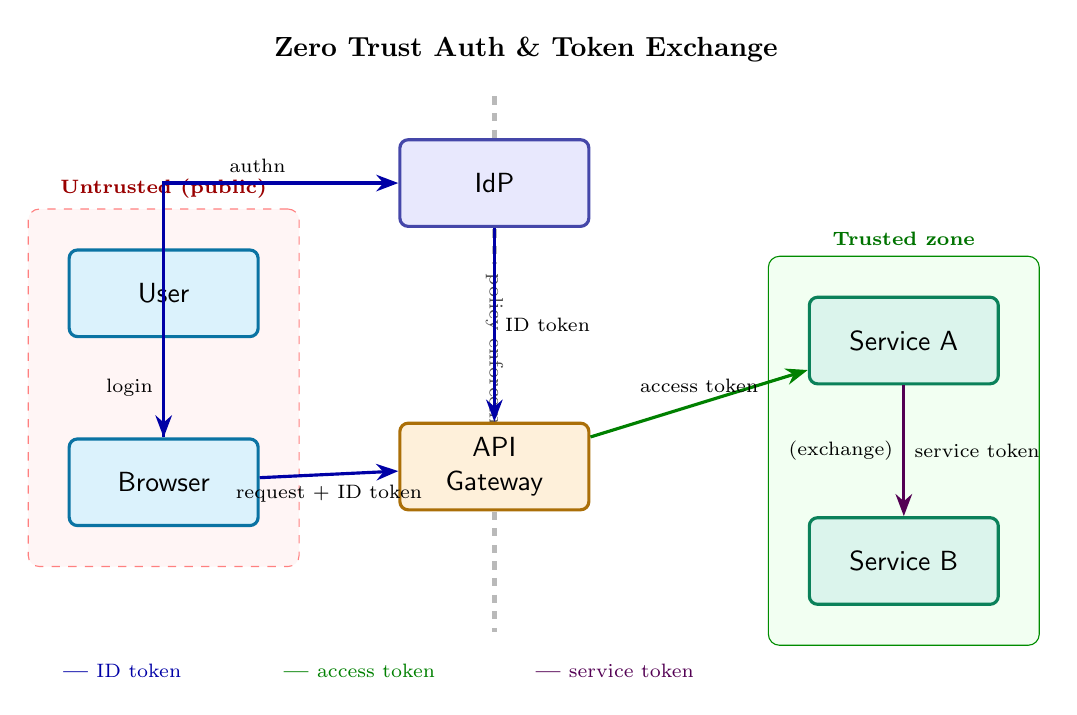
\begin{tikzpicture}[
  >={Stealth[length=2.8mm]},font=\sffamily,
  b/.style={rectangle,rounded corners=3pt,draw=#1!70!black,fill=#1!15,
            line width=0.4mm,minimum width=24mm,minimum height=11mm,align=center},
  idt/.style={->,line width=0.4mm,draw=blue!65!black},
  act/.style={->,line width=0.4mm,draw=green!50!black},
  svt/.style={->,line width=0.4mm,draw=violet!65!black},
]
  \definecolor{cclient}{HTML}{0EA5E9}
  \definecolor{cidp}{HTML}{6366F1}
  \definecolor{cgw}{HTML}{F59E0B}
  \definecolor{csvc}{HTML}{10B981}

  % clients (untrusted zone, left)
  \node[b=cclient] (user) at (0,5.2) {User};
  \node[b=cclient] (browser) at (0,2.8) {Browser};
  % IdP (top center)
  \node[b=cidp] (idp) at (4.2,6.6) {IdP};
  % gateway (boundary)
  \node[b=cgw] (gw) at (4.2,3.0) {API\\Gateway};
  % services (trusted zone, right)
  \node[b=csvc] (svcA) at (9.4,4.6) {Service A};
  \node[b=csvc] (svcB) at (9.4,1.8) {Service B};

  % flows
  \draw[idt] (user) -- node[left,font=\scriptsize]{login} (browser);
  \draw[idt] (browser.north) |- node[above,pos=0.7,font=\scriptsize]{authn} (idp.west);
  \draw[idt] (idp.south) -- node[right,font=\scriptsize]{ID token} (gw.north);
  \draw[act] (gw) -- node[above,font=\scriptsize]{access token} (svcA);
  \draw[svt] (svcA) -- node[right,font=\scriptsize]{service token}node[left,font=\scriptsize]{(exchange)} (svcB);
  \draw[idt] (browser) -- node[below,font=\scriptsize]{request + ID token} (gw);

  % token legend
  \node[anchor=west,font=\scriptsize,blue!65!black] at (-1.4,0.4) {\textbf{---} ID token};
  \node[anchor=west,font=\scriptsize,green!50!black] at (1.4,0.4) {\textbf{---} access token};
  \node[anchor=west,font=\scriptsize,violet!65!black] at (4.6,0.4) {\textbf{---} service token};

  % trust boundaries
  \begin{scope}[on background layer]
    \node[fit=(user)(browser),draw=red!50,dashed,rounded corners,inner sep=5mm,
          fill=red!4,label={[red!60!black,font=\scriptsize\bfseries]north:Untrusted (public)}] {};
    \node[fit=(svcA)(svcB),draw=green!55!black,rounded corners,inner sep=5mm,
          fill=green!5,label={[green!45!black,font=\scriptsize\bfseries]north:Trusted zone}] {};
    \draw[gray!55,line width=0.6mm,dashed] (4.2,7.7) -- (4.2,0.9)
        node[pos=0.5,fill=white,font=\scriptsize,text=gray!60!black,sloped] {policy enforcement};
  \end{scope}

  \node[font=\bfseries] at (4.6,8.3) {Zero Trust Auth \& Token Exchange};
\end{tikzpicture}
\end{document}
